\documentclass[12pt]{article}
\usepackage{fullpage}
\usepackage{graphicx}
\usepackage{amsmath, amssymb}
\usepackage{listings}
\usepackage{xcolor}
\usepackage{hyperref}
\usepackage{float}
% Define colors for the code listings
\definecolor{mygreen}{rgb}{0,0.6,0}
\definecolor{mygray}{rgb}{0.5,0.5,0.5}
\definecolor{mymauve}{rgb}{0.58,0,0.82}

% Setup for the C code listing style
\lstset{ %
  backgroundcolor=\color{white},   
  basicstyle=\footnotesize\ttfamily,  
  breaklines=true,                   
  captionpos=b,                      
  commentstyle=\color{mygreen},      
  keywordstyle=\color{blue},         
  stringstyle=\color{mymauve},       
  numbers=left,                      
  numbersep=5pt,                     
  numberstyle=\tiny\color{mygray},
  frame=single,
  language=C
}

\title{Digital Clock Project Report}
\author{Mohit}
\date{\today}

\begin{document}
\maketitle
\tableofcontents
\newpage

\section{Introduction}
This report describes the design and implementation of a digital clock using an ATmega328P microcontroller (the heart of an Arduino Uno), a SN7447 BCD-to-seven-segment decoder/driver, and six common-anode seven-segment displays. Two push buttons allow the user to adjust the clock’s hours and minutes. The design uses a multiplexing technique to drive all displays with a single SN7447 and directly controlled microcontroller outputs.

\section{Hardware Components and Their Roles}
\subsection{ATmega328P (Arduino Uno)}
The ATmega328P acts as the central controller for the clock. It:
\begin{itemize}
    \item Generates 4-bit Binary Coded Decimal (BCD) signals to be sent to the SN7447.
    \item Controls which display is active via multiplexing.
    \item Reads the state of push buttons to adjust the time.
\end{itemize}

\subsection{SN7447 BCD-to-Seven-Segment Decoder/Driver}
The SN7447 decodes the 4-bit BCD input into the corresponding segment control signals for a seven-segment display. It is designed for common-anode displays, and its outputs are connected (via current-limiting resistors) in parallel to the segments of all six displays.

\subsection{Seven-Segment Displays}
Six common-anode seven-segment displays are used to show the time in HH:MM:SS format. Because only one SN7447 is used, the displays are multiplexed by sequentially activating each digit's common anode.

\subsection{Resistors}
\begin{itemize}
    \item \textbf{Current-Limiting Resistors:} Each segment of every display is connected through a resistor (typically 220–330\(\Omega\)) to limit the LED current.
    \item \textbf{Internal Pull-Up Resistors:} Enabled in software for the push buttons.
\end{itemize}

\subsection{Push Buttons}
Two push buttons are used:
\begin{itemize}
    \item One for adjusting the hour.
    \item One for adjusting the minute.
\end{itemize}
They are wired between the microcontroller input pins and ground, utilizing the Arduino’s internal pull-up resistors.

\section{Circuit Connections}
\subsection{Power and Ground}
\begin{itemize}
    \item The Arduino’s regulated 5V output powers the SN7447 and the displays.
    \item All ground lines (Arduino, SN7447, displays, and push buttons) are connected to a common ground.
\end{itemize}

\subsection{SN7447 Connections}
\begin{itemize}
    \item \textbf{BCD Inputs:}  
    Arduino digital pins 2, 3, 4, and 5 (mapped to PD2, PD3, PD4, and PD5 respectively) connect to the SN7447's BCD input pins.
    \item \textbf{Segment Outputs:}  
    The outputs for segments \textit{a} through \textit{g} from the SN7447 are connected to all six seven-segment displays through individual current-limiting resistors.
\end{itemize}

\subsection{Multiplexing and Digit Selection}
Since only one SN7447 is used, the displays are multiplexed:
\begin{itemize}
    \item Each display’s common anode is directly connected to a microcontroller output pin.
    \item Pin assignments for digit selection are as follows:
    \begin{itemize}
        \item Digit 1 (tens of hours): Arduino digital pin 6 (PD6)
        \item Digit 2 (ones of hours): Arduino digital pin 7 (PD7)
        \item Digit 3 (tens of minutes): Arduino digital pin 8 (PB0)
        \item Digit 4 (ones of minutes): Arduino digital pin 9 (PB1)
        \item Digit 5 (tens of seconds): Arduino digital pin 10 (PB2)
        \item Digit 6 (ones of seconds): Arduino digital pin 11 (PB3)
    \end{itemize}
    \item The microcontroller rapidly cycles through these outputs (multiplexing) so that all digits appear continuously lit.
\end{itemize}

\subsection{Push Button Connections}
\begin{itemize}
    \item \textbf{Hour Adjust Button:}  
    Connected between Arduino digital pin 12 (PB4) and ground, configured as an input with an internal pull-up.
    \item \textbf{Minute Adjust Button:}  
    Connected between Arduino digital pin 13 (PB5) and ground, also configured with an internal pull-up.
\end{itemize}

\section{Software Implementation and Code Explanation}
The code is written in pure AVR C (using \texttt{avr-gcc}) and runs on the ATmega328P. It includes the following standard libraries:
\begin{itemize}
    \item \textbf{\texttt{<avr/io.h>}}: Provides access to the microcontroller's registers (PORT, DDR, and PIN) for I/O operations.
    \item \textbf{\texttt{<util/delay.h>}}: Offers the \texttt{\_delay\_ms()} function for creating time delays necessary for multiplexing and debouncing.
    \item \textbf{\texttt{<stdint.h>}}: Supplies standard integer types (e.g., \texttt{uint8\_t}) for portability.
\end{itemize}

\subsection{Code Structure}
\subsubsection{Initialization}
\begin{itemize}
    \item \textbf{I/O Configuration:}  
    The BCD output pins (PD2–PD5) are set as outputs. Digit select pins on PORTD (PD6, PD7) and PORTB (PB0--PB3) are also configured as outputs. The push button pins (PB4, PB5) are configured as inputs with enabled pull-ups.
    \item \textbf{Clock Variables:}  
    Variables for hours, minutes, and seconds are initialized (default starting time: 12:00:00). A cycle counter is used to approximate a one-second interval based on the multiplexing delay.
\end{itemize}

\subsubsection{Multiplexing the Display}
\begin{itemize}
    \item The current time is broken into six individual digits (HH:MM:SS).
    \item The code loops through each digit, sending the corresponding 4-bit BCD value to the SN7447 via PORTD (PD2--PD5).
    \item Only one display is activated at a time by setting the corresponding digit select pin HIGH.
    \item A short delay (e.g., 2ms) allows the digit to be visible before deactivating the display and moving to the next.
    \item Rapid cycling (multiplexing) creates the illusion that all six digits are lit simultaneously.
\end{itemize}

\subsubsection{Timekeeping and Button Handling}
\begin{itemize}
    \item \textbf{Software Timekeeping:}  
    A cycle counter increments with each complete multiplex cycle. When the counter reaches approximately 83 cycles (around 1 second), the seconds variable is incremented. When seconds, minutes, or hours reach their limits (60 or 24), the variables are reset and the next unit is incremented.
    \item \textbf{Push Button Adjustments:}  
    The code polls the push button inputs. When a button is pressed (detected by a LOW signal), a debounce delay is introduced, and the corresponding time variable (hours or minutes) is incremented. The system waits until the button is released before continuing.
\end{itemize}

\subsection{Complete Code Listing}
\begin{lstlisting}[caption={Digital Clock Code in AVR C}, label=lst:clock]
/*
 * Digital Clock using 6 seven-segment displays with SN7447 driver
 * ATmega328P (Arduino Uno) version in pure C for avr-gcc
 *
 * Pin Mapping:
 *   BCD outputs (to SN7447): Arduino pins 2-5  => PD2, PD3, PD4, PD5
 *   Digit Select outputs:
 *      Digit 1 (tens of hours): pin 6  => PD6
 *      Digit 2 (ones of hours):  pin 7  => PD7
 *      Digit 3 (tens of minutes):pin 8  => PB0
 *      Digit 4 (ones of minutes):pin 9  => PB1
 *      Digit 5 (tens of seconds):pin 10 => PB2
 *      Digit 6 (ones of seconds):pin 11 => PB3
 *   Push Buttons:
 *      Hour adjust:   pin 12 => PB4 (input with pull-up)
 *      Minute adjust: pin 13 => PB5 (input with pull-up)
 */

#include <avr/io.h>
#include <util/delay.h>
#include <stdint.h>

#define DIGIT_DELAY_MS 2    // Delay per digit in milliseconds
#define NUM_DIGITS 6

int main(void) {
    // I/O Setup
    DDRD |= (1 << PD2) | (1 << PD3) | (1 << PD4) | (1 << PD5); // BCD outputs
    DDRD |= (1 << PD6) | (1 << PD7);                            // Digit select: digits 1 & 2
    DDRB |= (1 << PB0) | (1 << PB1) | (1 << PB2) | (1 << PB3);    // Digit select: digits 3 to 6

    // Configure push buttons on PB4 and PB5 as inputs with pull-ups
    DDRB &= ~((1 << PB4) | (1 << PB5));  
    PORTB |= (1 << PB4) | (1 << PB5);

    // Initialize clock variables (12:00:00)
    uint8_t hours = 12;
    uint8_t minutes = 0;
    uint8_t seconds = 0;
    uint16_t cycle_count = 0;  // For approximating a 1-second interval

    while (1) {
        // Break time into individual digits: HH:MM:SS
        uint8_t digits[NUM_DIGITS];
        digits[0] = hours / 10;       // Tens of hours
        digits[1] = hours % 10;       // Ones of hours
        digits[2] = minutes / 10;     // Tens of minutes
        digits[3] = minutes % 10;     // Ones of minutes
        digits[4] = seconds / 10;     // Tens of seconds
        digits[5] = seconds % 10;     // Ones of seconds

        // Multiplex through each digit
        for (uint8_t i = 0; i < NUM_DIGITS; i++) {
            // Set BCD outputs: Clear PD2-PD5 and set new value
            PORTD = (PORTD & ~0x3C) | ((digits[i] << 2) & 0x3C);
            
            // Activate corresponding digit
            if (i < 2) {
                if (i == 0)
                    PORTD |= (1 << PD6);  // Activate digit 1 (tens of hours)
                else
                    PORTD |= (1 << PD7);  // Activate digit 2 (ones of hours)
            } else {
                PORTB |= (1 << (i - 2));   // Activate digits 3-6 (PB0-PB3)
            }
            _delay_ms(DIGIT_DELAY_MS);  // Allow digit to be visible

            // Deactivate digit
            if (i < 2) {
                if (i == 0)
                    PORTD &= ~(1 << PD6);
                else
                    PORTD &= ~(1 << PD7);
            } else {
                PORTB &= ~(1 << (i - 2));
            }
        } // End multiplexing

        cycle_count++;

        // Check push buttons for time adjustment
        if (!(PINB & (1 << PB4))) { // Hour adjustment button pressed
            _delay_ms(50);
            if (!(PINB & (1 << PB4))) {
                hours = (hours + 1) % 24;
                while (!(PINB & (1 << PB4)));
                _delay_ms(50);
            }
        }
        if (!(PINB & (1 << PB5))) { // Minute adjustment button pressed
            _delay_ms(50);
            if (!(PINB & (1 << PB5))) {
                minutes = (minutes + 1) % 60;
                while (!(PINB & (1 << PB5)));
                _delay_ms(50);
            }
        }

        // Update time approximately every 83 multiplex cycles (approx. 1 second)
        if (cycle_count >= 83) {
            cycle_count = 0;
            seconds++;
            if (seconds >= 60) {
                seconds = 0;
                minutes++;
                if (minutes >= 60) {
                    minutes = 0;
                    hours++;
                    if (hours >= 24)
                        hours = 0;
                }
            }
        }
    } // End main loop

    return 0;
}
\end{lstlisting}

\begin{figure}[H]
    \centering
        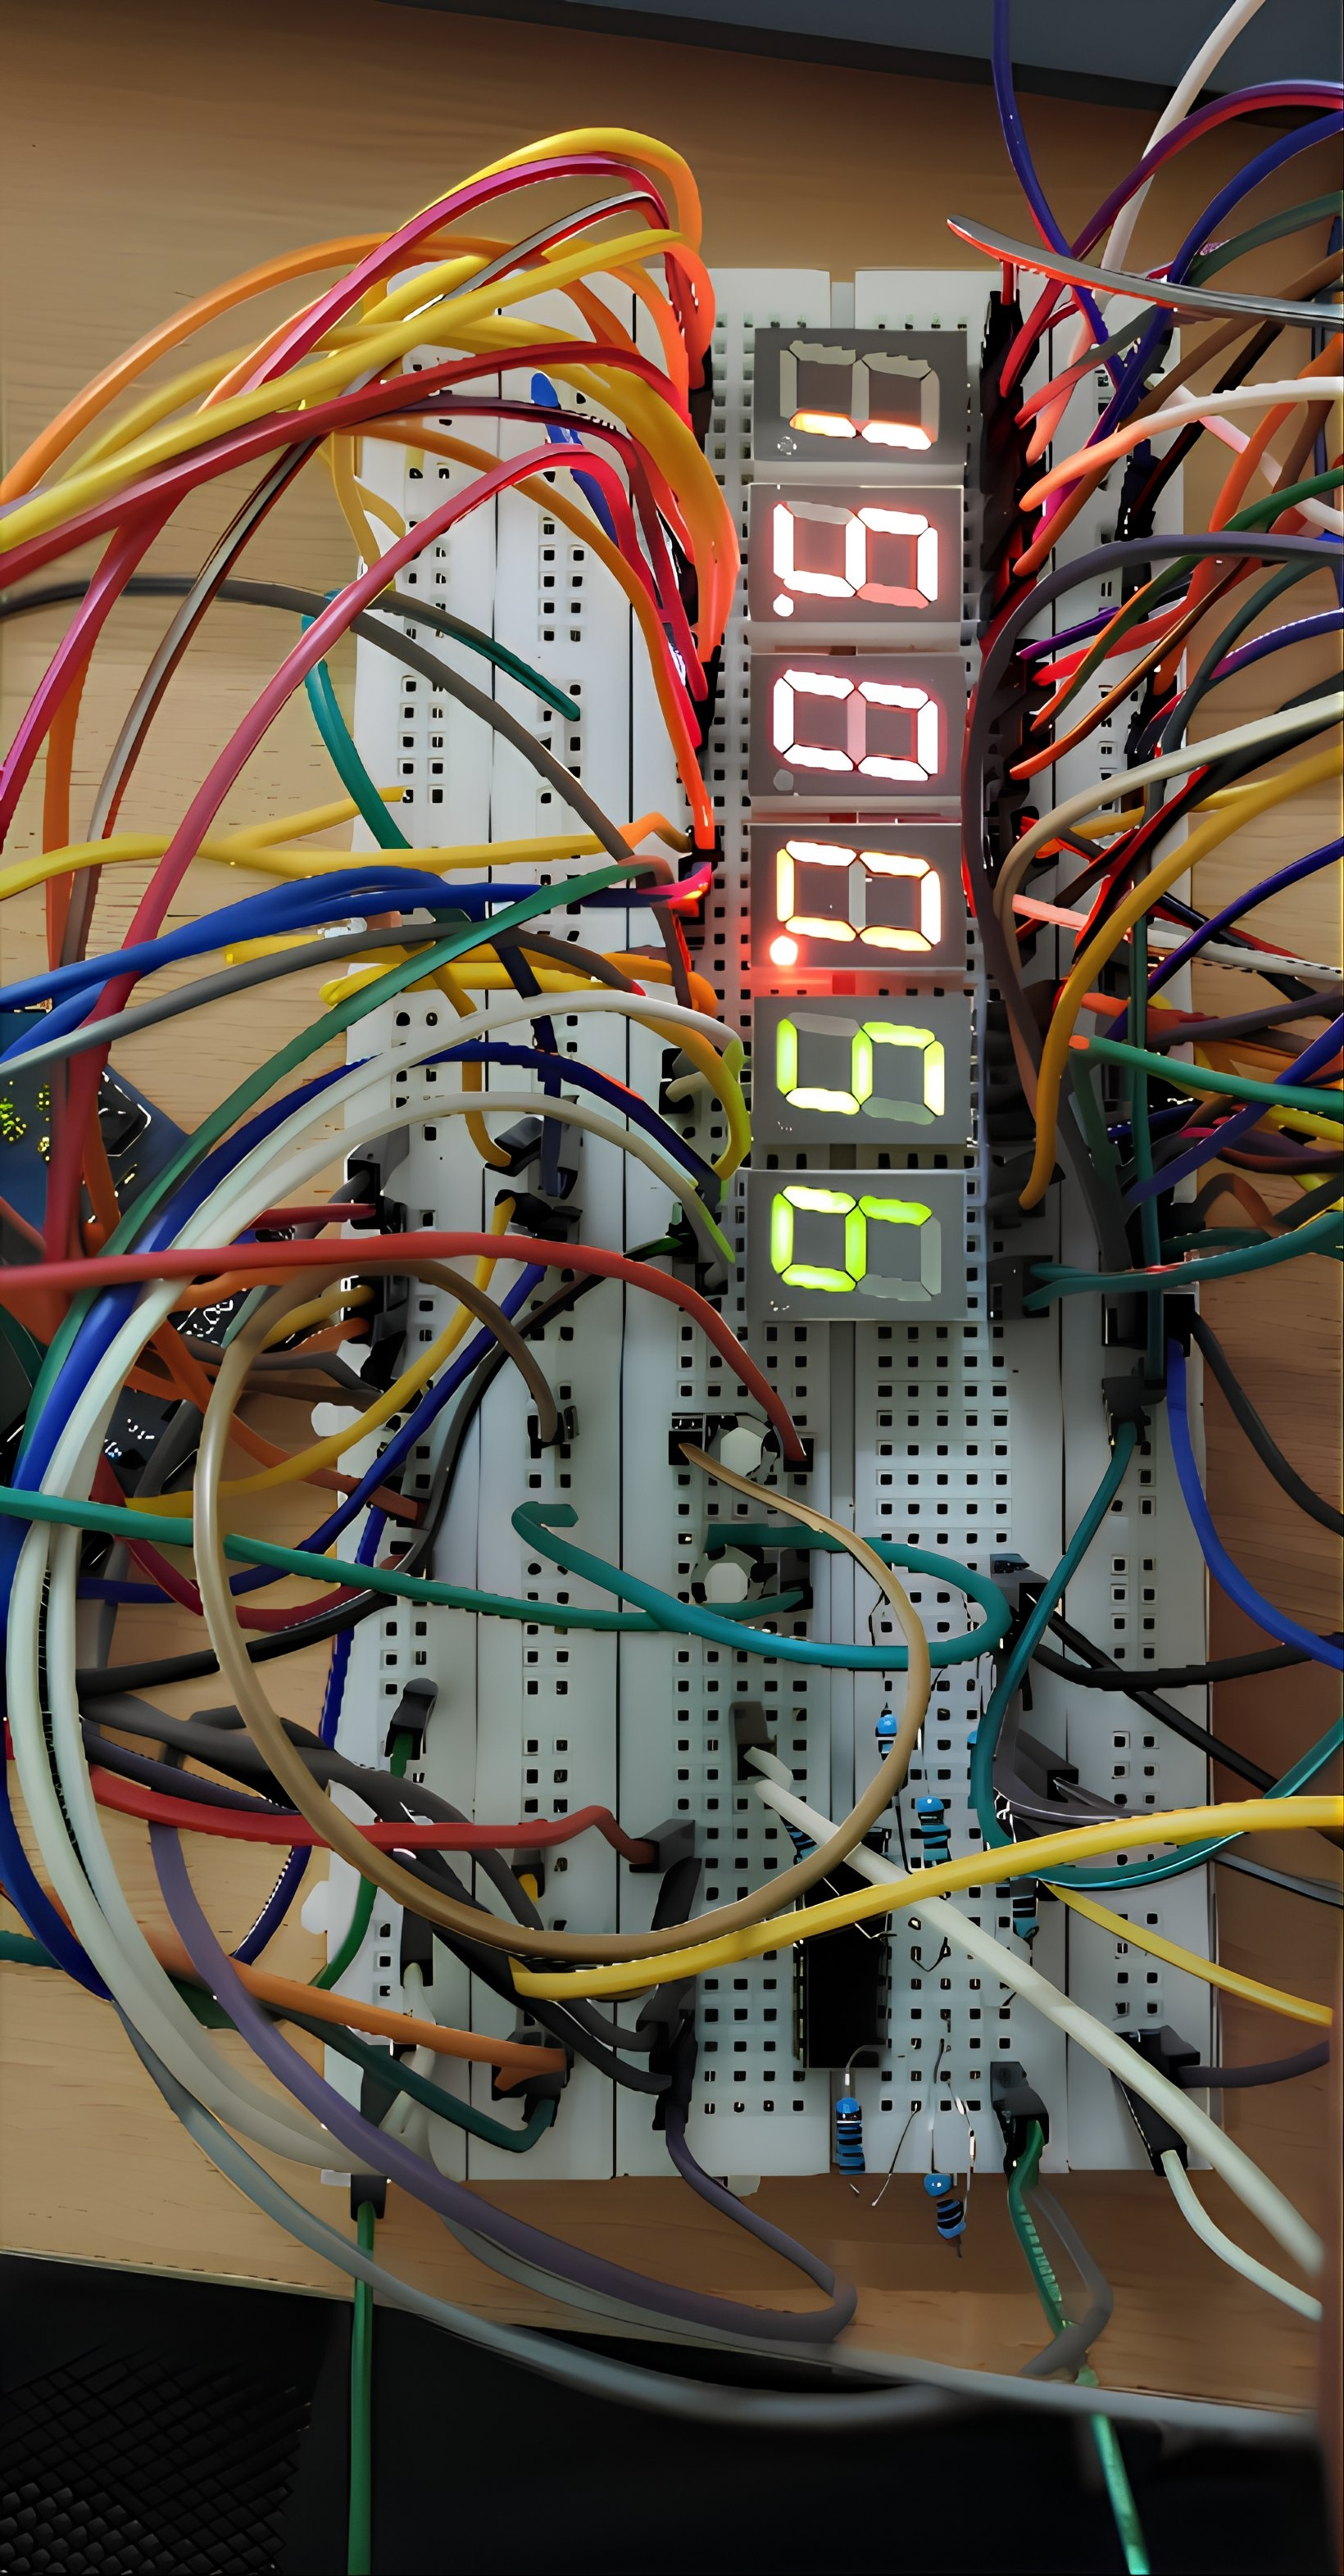
\includegraphics[height=8cm]{figs/IMG_20250323_143858.jpg}
\end{figure}

\section{Conclusion}
This project demonstrates how a digital clock can be implemented using minimal hardware by employing multiplexing techniques and a dedicated BCD-to-seven-segment decoder. The ATmega328P directly controls the SN7447 and the displays while handling timekeeping and user input via push buttons. The software, written in pure AVR C, efficiently manages the hardware through direct register manipulation and software delays. This report provides a comprehensive understanding of the hardware connections and the software architecture required to build and operate a digital clock.

\end{document}
---
